\section{CPD}


\begin{figure}[!htbp]
\minipage{0.5\textwidth}%
\centering
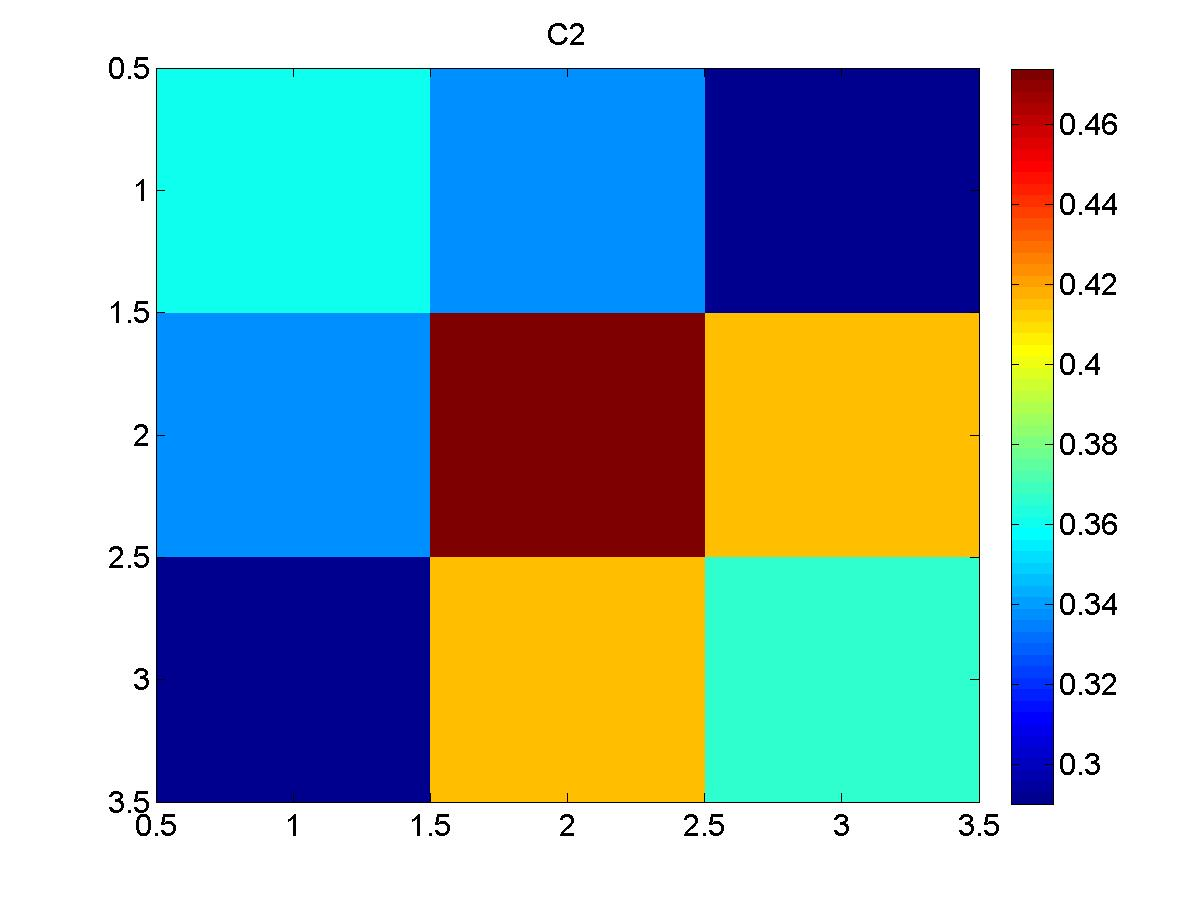
\includegraphics[width=1\linewidth]{400.jpg}
\subcaption{Covariance matrix (2x2)}
\endminipage\hfill
\minipage{0.5\textwidth}%
\centering
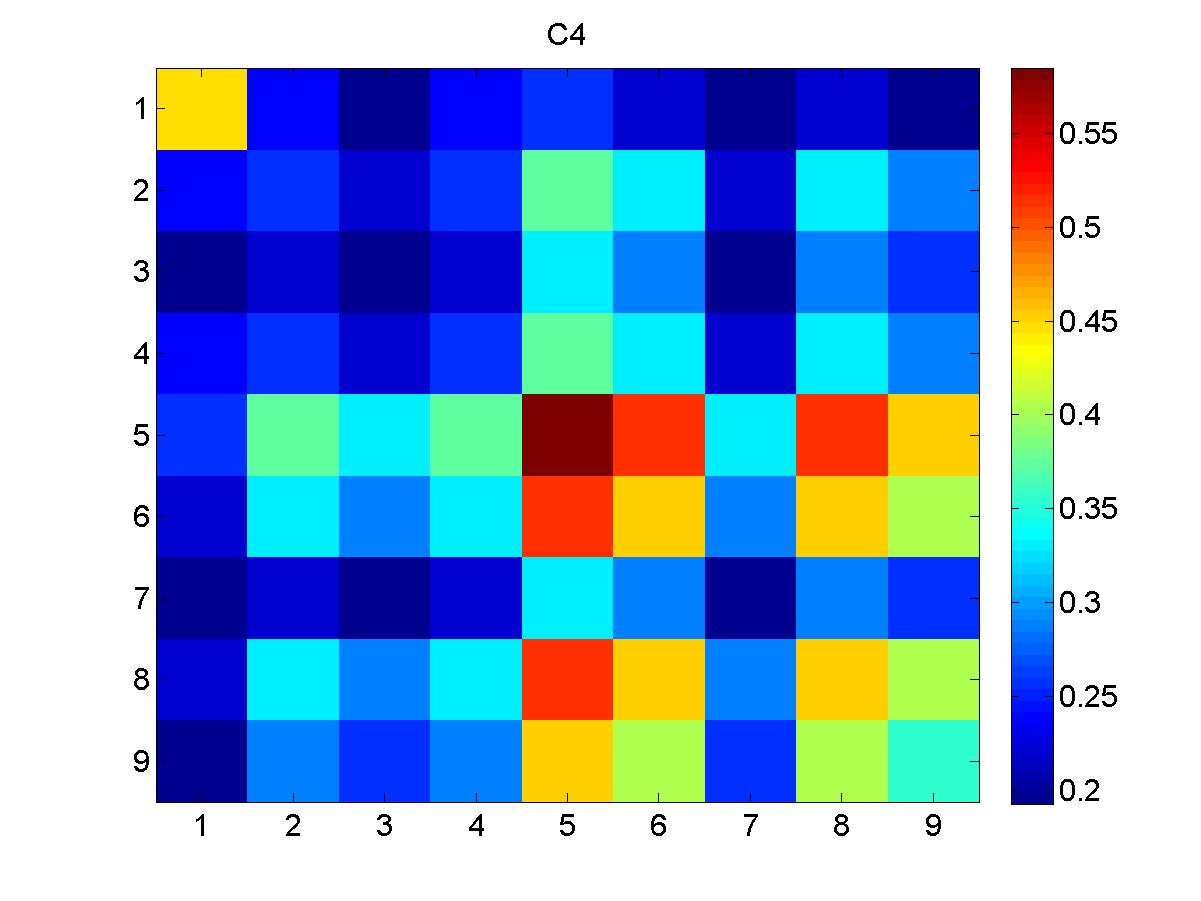
\includegraphics[width=1\linewidth]{401.jpg}
\subcaption{Fourth order cumulative tensor (3x3x3x3) stretched at (9x9).}
\endminipage\hfill
\caption{Tensors overview}
\end{figure}

Their rank is estimated to be two for both cases and the number of dimensions (order) for the first and the second tensor are respectively two and four. The CPD relation for this will be as equation \ref{C2} and \ref{C4} respectively to C2 and C4 dataset.

\begin{equation}\label{C2}
    C2=\sum_{r=1}^{2} U_{r}^{(1)}\otimes U_{r}^{(1)}
\end{equation}

\begin{equation}\label{C4}
    C4=\sum_{r=1}^{2} U_{r}^{(1)}\otimes U_{r}^{(2)}\otimes U_{r}^{(3)}\otimes U_{r}^{(4)}}
\end{equation}

Alternatively this could be re-written into a rang $(L_{r},L_{r},1)$ of a block term decomposition as in the equation \ref{BTD}

\begin{equation}\label{BTD}
    Tensor=A(C\Theta B)^{T}
\end{equation}

where $\Theta$ is Khatri–Rao product of tensors. This is a suitable notation for alternative least square algorithm. The component A,B and C component for tensor C2 and C4 are respectively in figure \ref{C22} and \ref{C44}. 

\begin{figure}[!htbp]
\minipage{0.33\textwidth}%
\centering
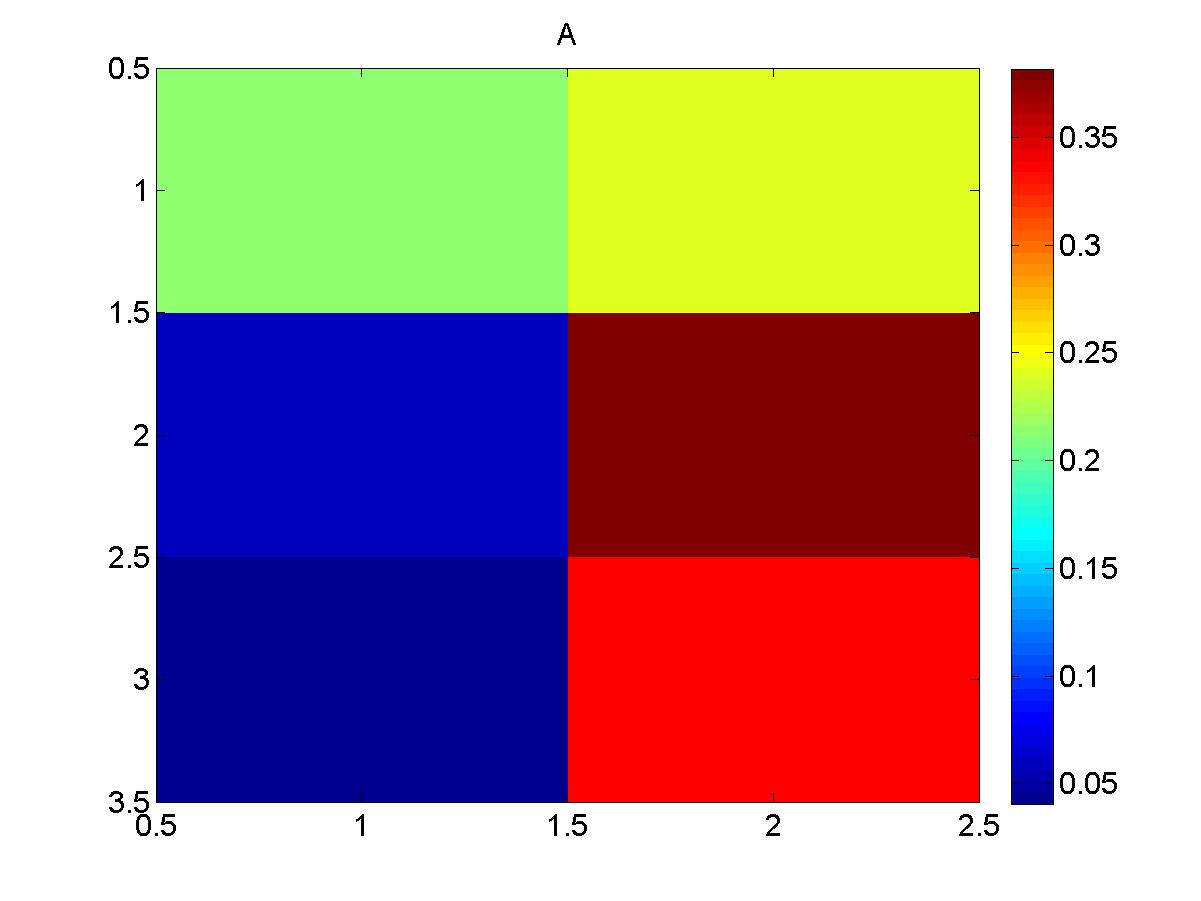
\includegraphics[width=1\linewidth]{402.jpg}
\subcaption{A component.}
\endminipage\hfill
\minipage{0.33\textwidth}%
\centering
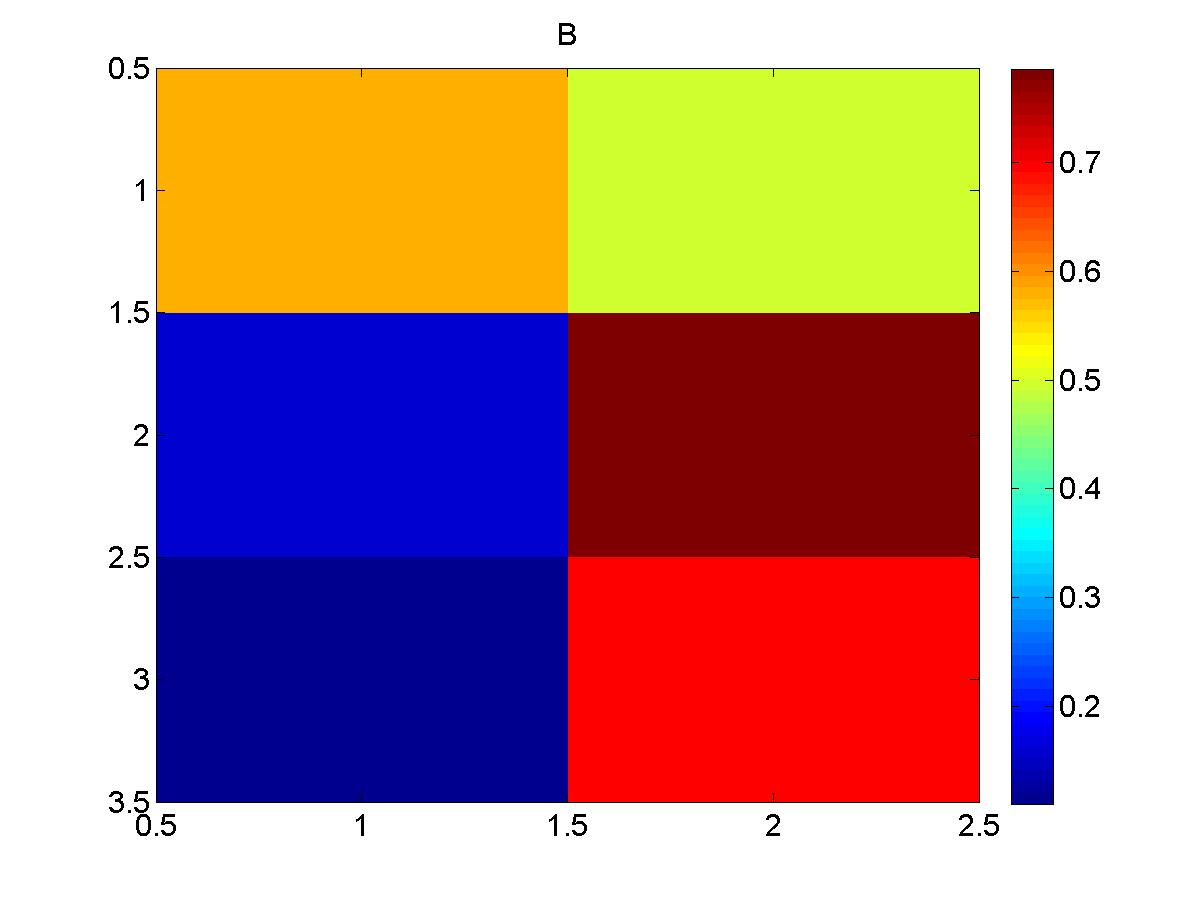
\includegraphics[width=1\linewidth]{403.jpg}
\subcaption{B component}
\endminipage\hfill
\minipage{0.33\textwidth}%
\centering
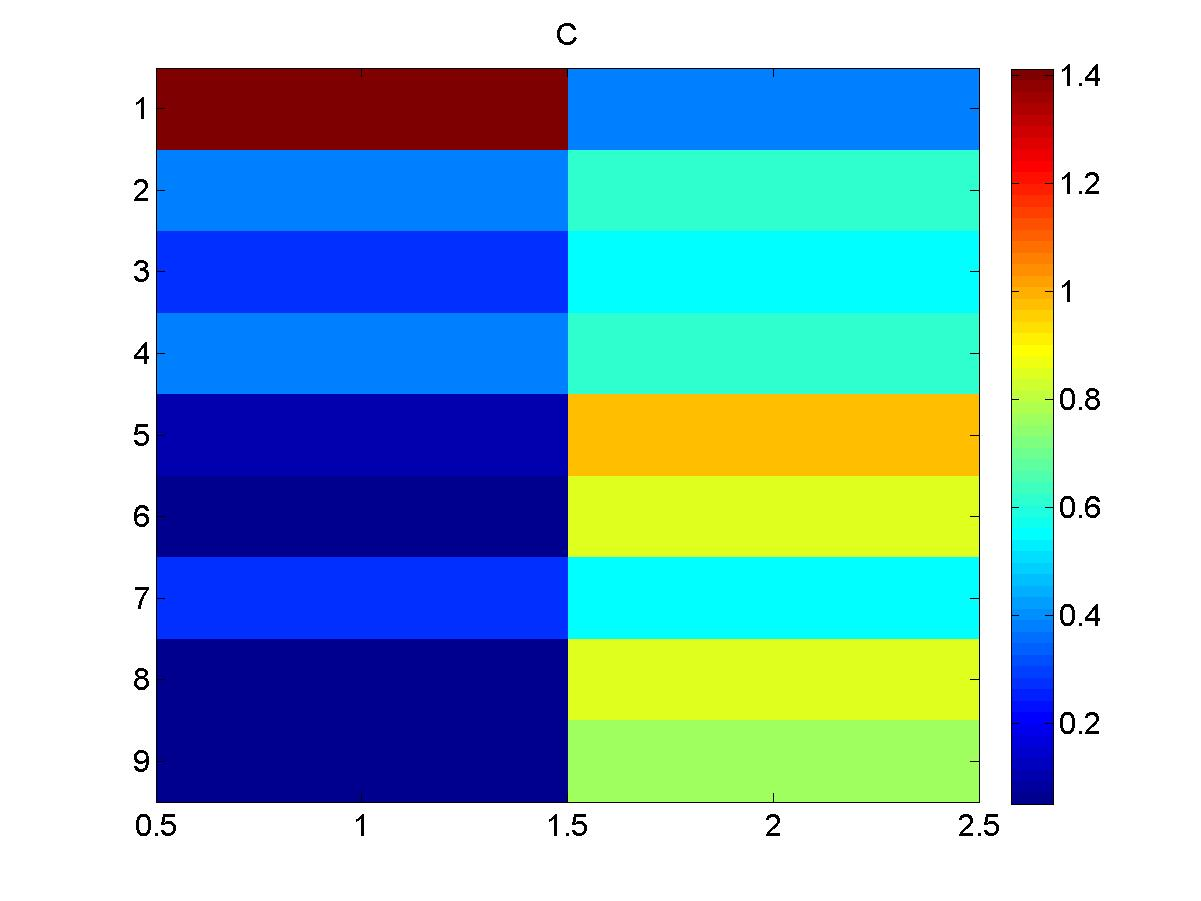
\includegraphics[width=1\linewidth]{404.jpg}
\subcaption{C component}
\endminipage\hfill
\caption{CPD decomposition of C2 matrix}\label{C22}
\end{figure}




\begin{figure}[!htbp]
\minipage{0.33\textwidth}%
\centering
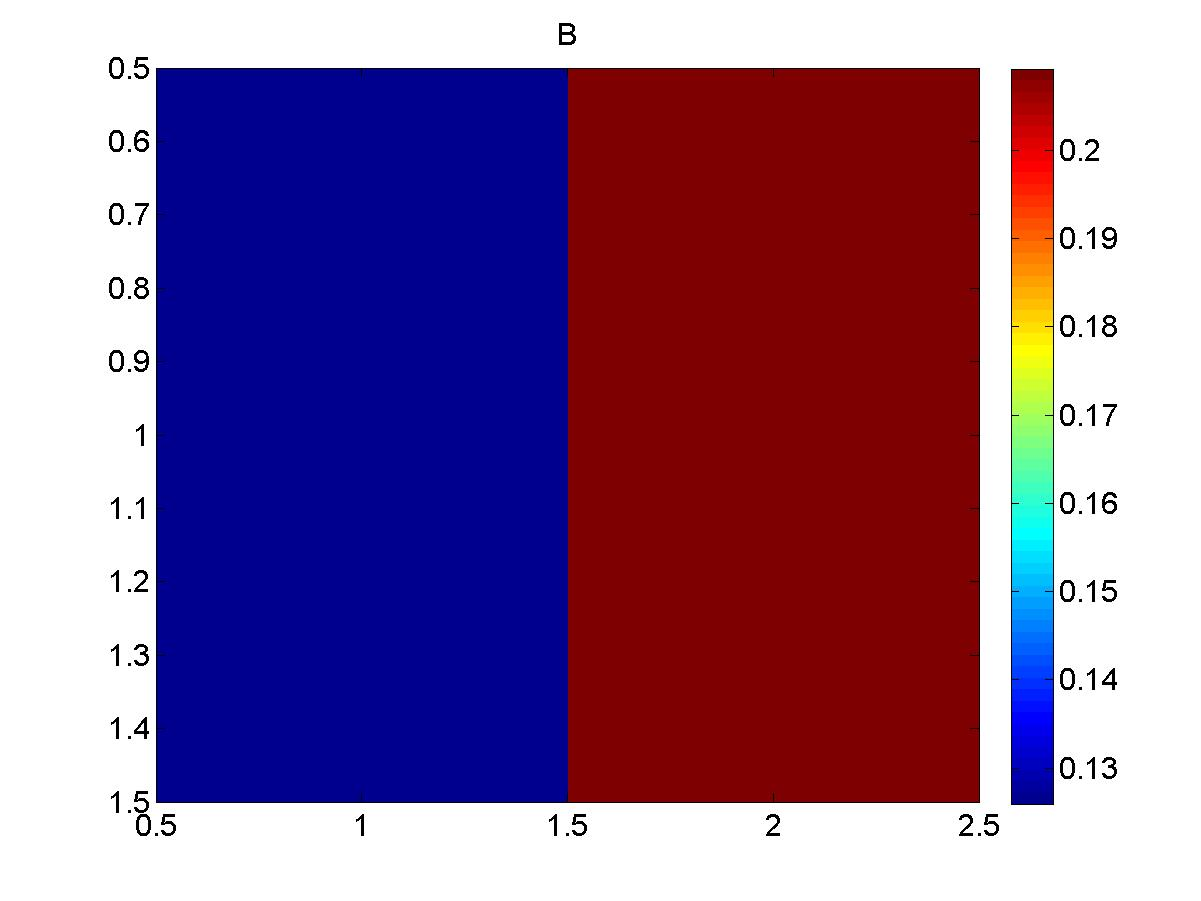
\includegraphics[width=1\linewidth]{405.jpg}
\subcaption{A component.}
\endminipage\hfill
\minipage{0.33\textwidth}%
\centering
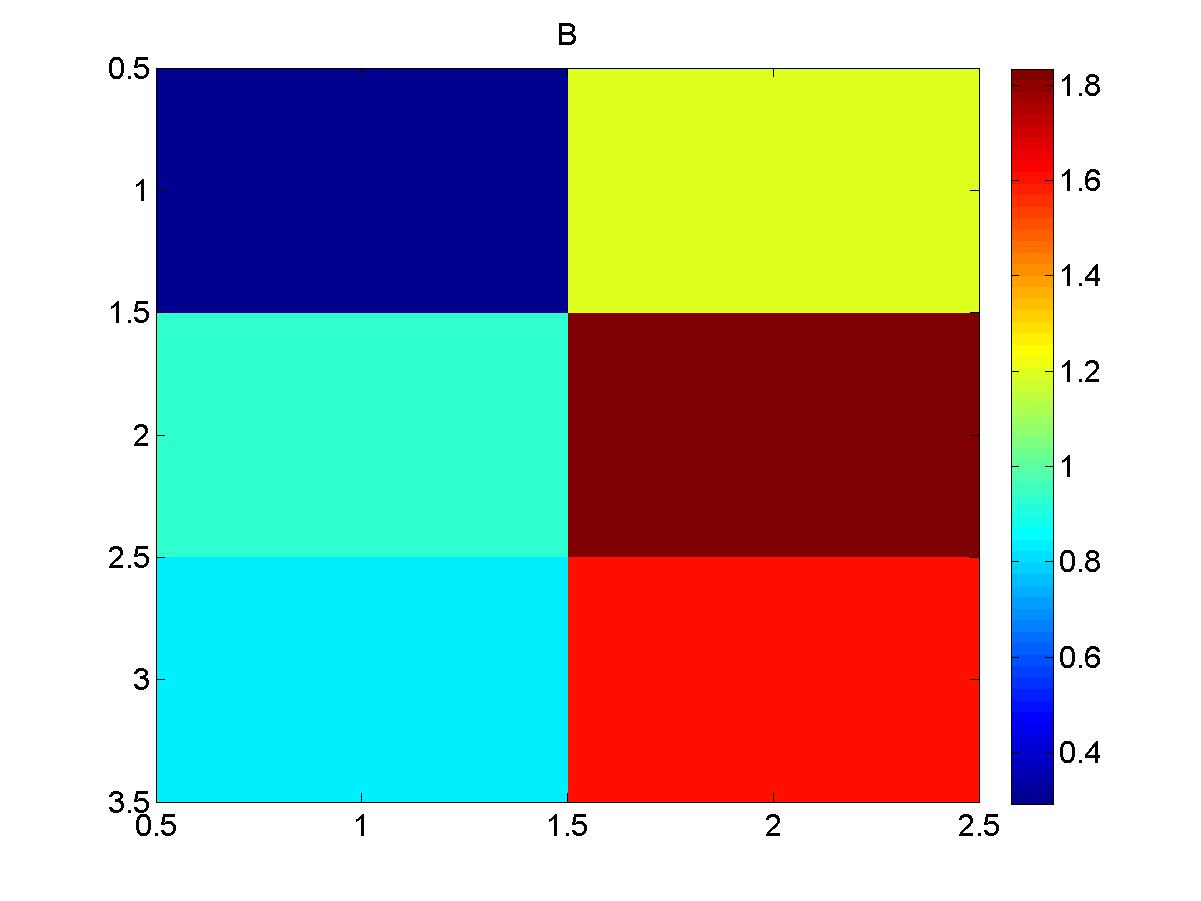
\includegraphics[width=1\linewidth]{406.jpg}
\subcaption{B component.}
\endminipage\hfill
\minipage{0.33\textwidth}%
\centering
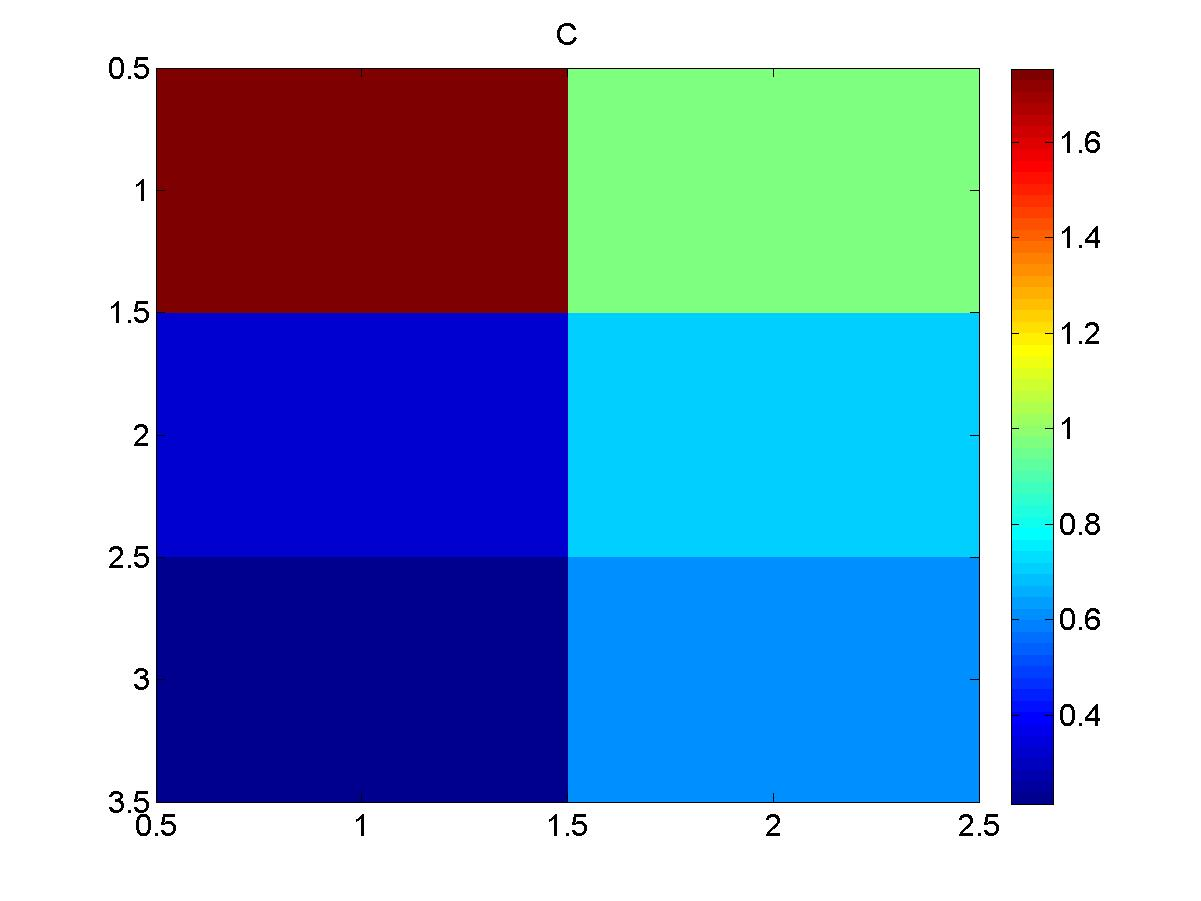
\includegraphics[width=1\linewidth]{407.jpg}
\subcaption{C component.}
\endminipage\hfill
\caption{CPD decomposition of C4 tensor}\label{C44}
\end{figure}


Tensorlab toolbox has also been utilized to do the rank estimation and the CPD decomposition. The matrices U from equation \ref{C2} and \ref{C4} are plotted in figures \ref{C222} and \ref{C444} respectively.



\begin{figure}[!htbp]
\minipage{0.5\textwidth}%
\centering
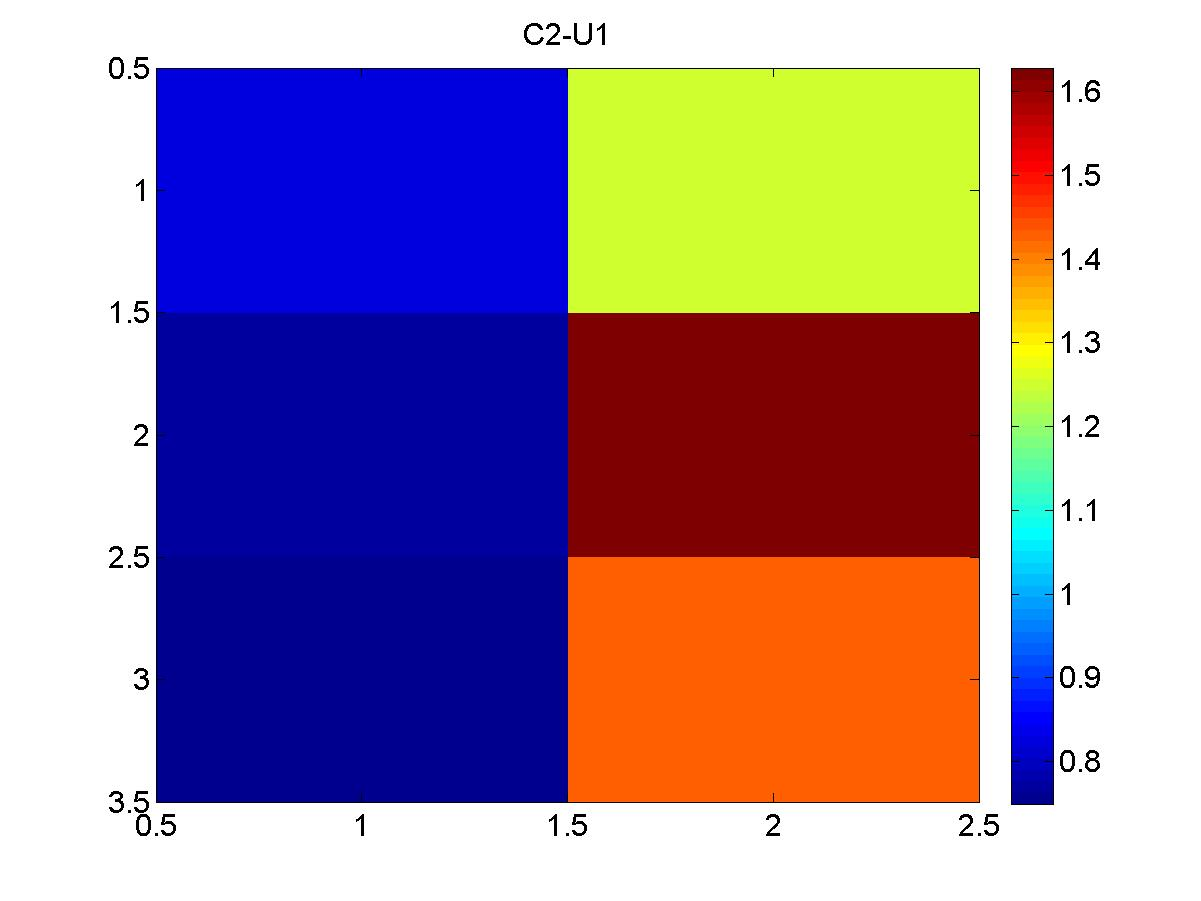
\includegraphics[width=1\linewidth]{408.jpg}
\subcaption{U1 component.}
\endminipage\hfill
\minipage{0.5\textwidth}%
\centering
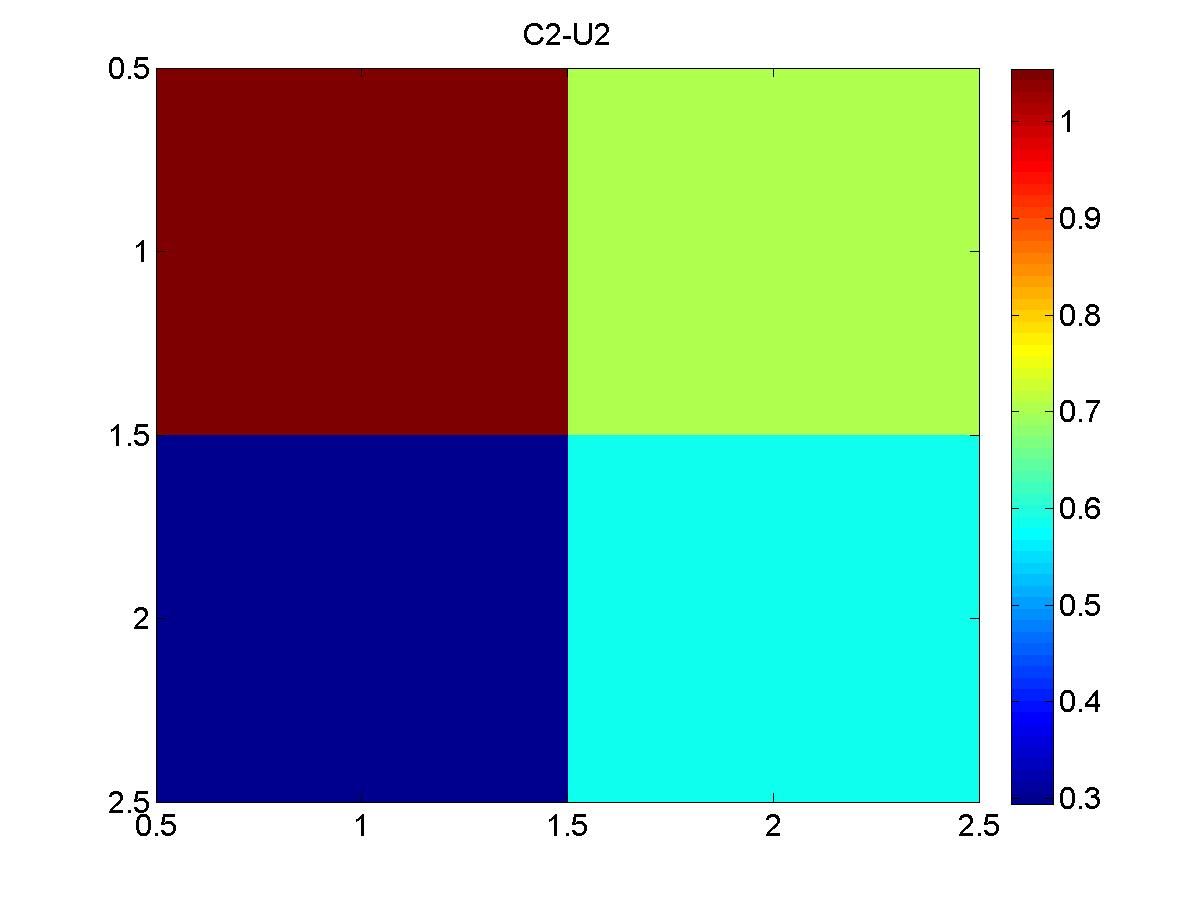
\includegraphics[width=1\linewidth]{409.jpg}
\subcaption{U2 component.}
\endminipage\hfill
\caption{CPD decomposition of C2 matrix}\label{C222}
\end{figure}


\begin{figure}[!htbp]
\minipage{0.5\textwidth}%
\centering
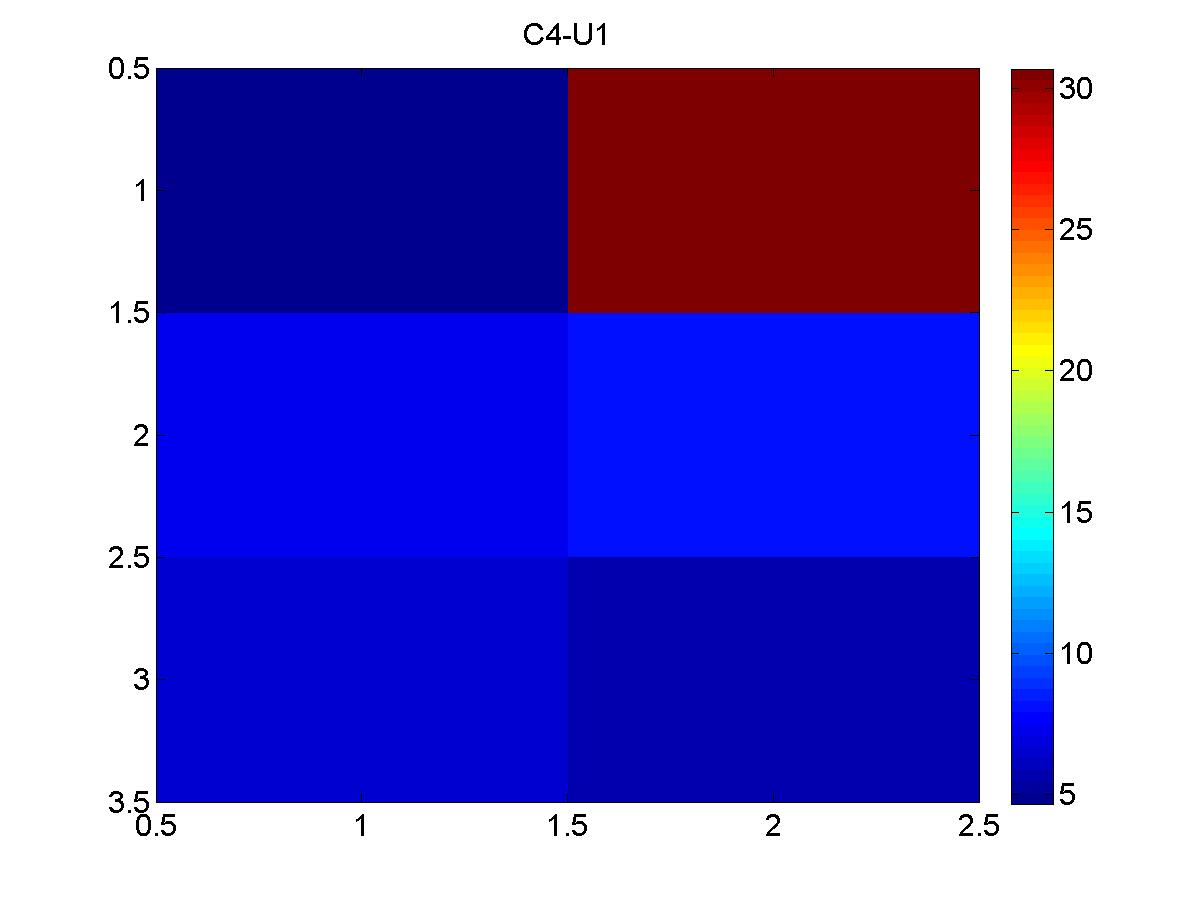
\includegraphics[width=1\linewidth]{410.jpg}
\subcaption{U1 component.}
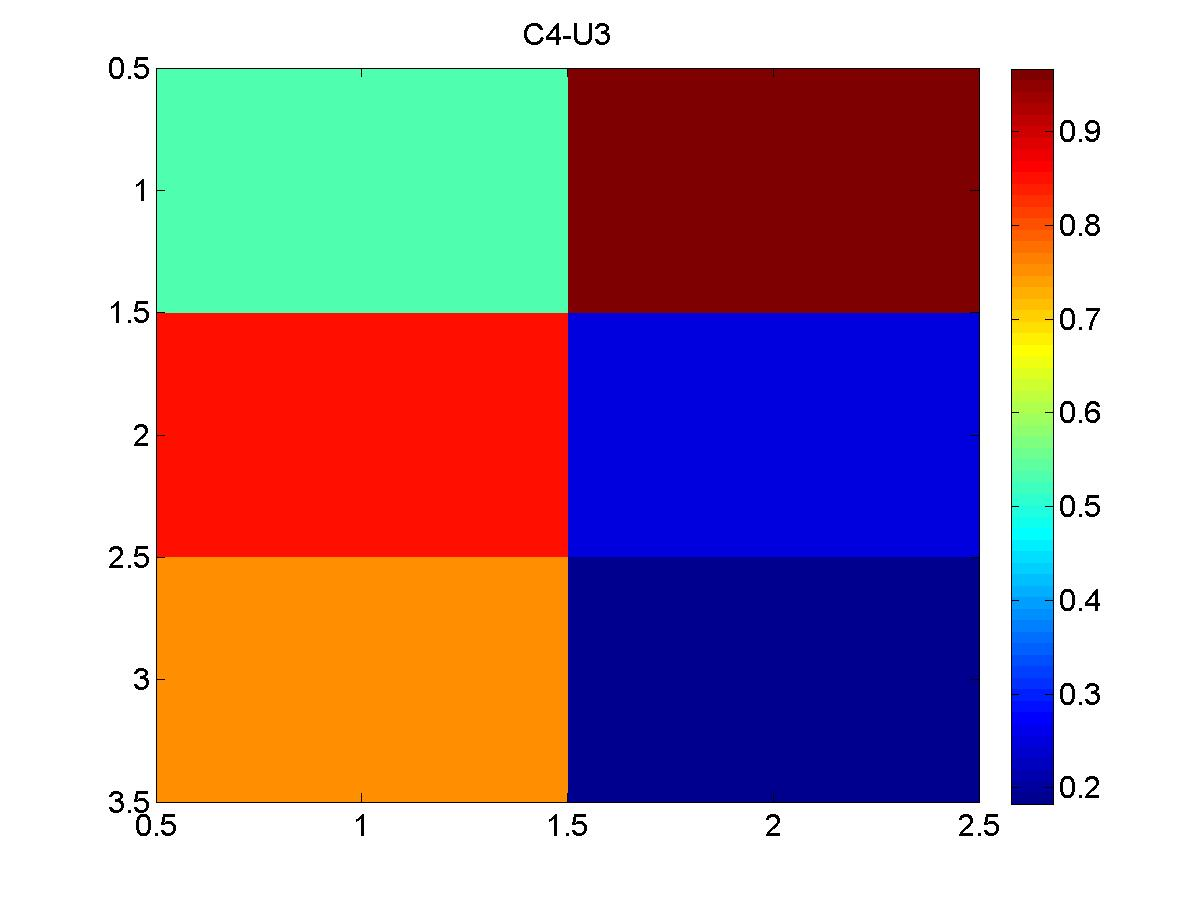
\includegraphics[width=1\linewidth]{412.jpg}
\subcaption{U3 component.}
\endminipage\hfill
\minipage{0.5\textwidth}%
\centering
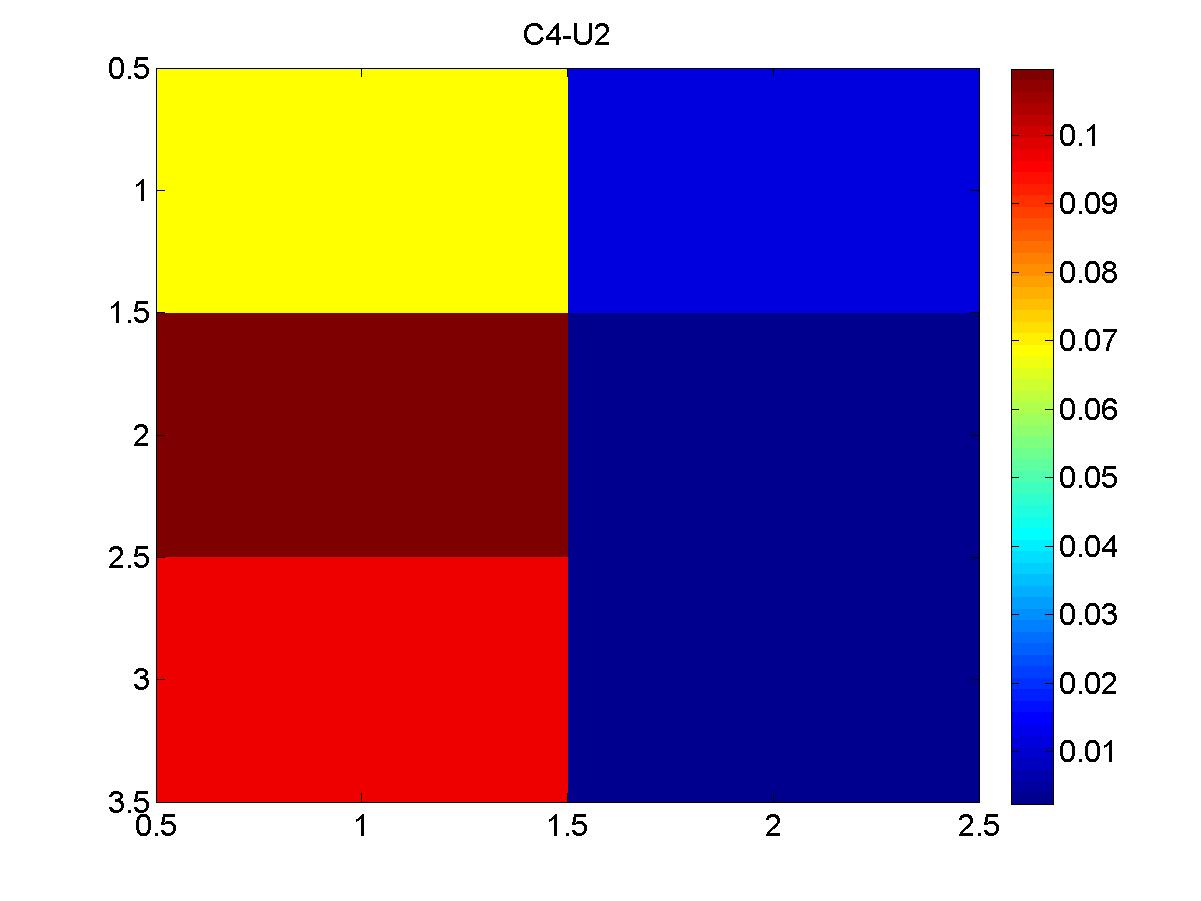
\includegraphics[width=1\linewidth]{411.jpg}
\subcaption{U2 component.}
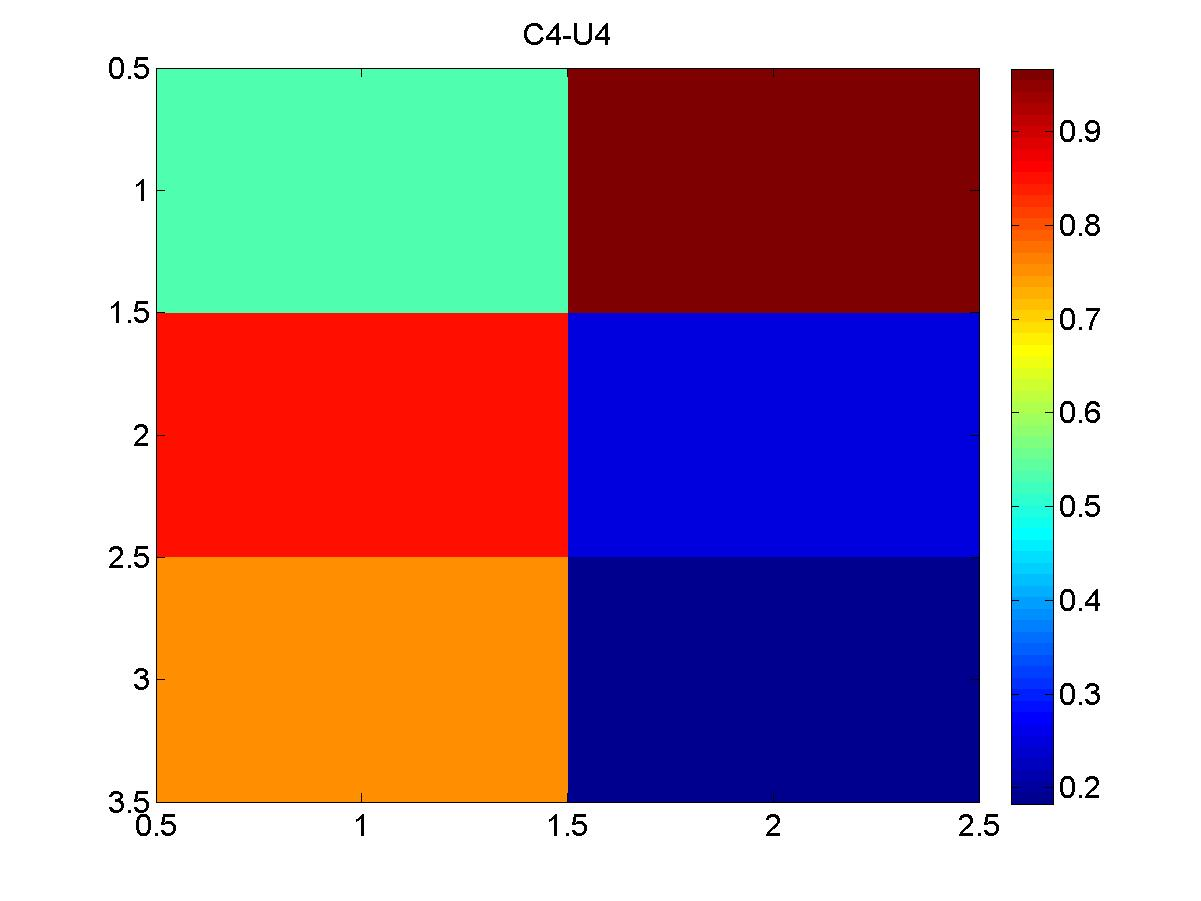
\includegraphics[width=1\linewidth]{413.jpg}
\subcaption{U4 component.}
\endminipage\hfill
\caption{CPD decomposition of C4 matrix}\label{C444}
\end{figure}
